\section{eo\-Perf2Worth\-Cached$<$ EOT, Worth\-T $>$ Class Template Reference}
\label{classeo_perf2_worth_cached}\index{eoPerf2WorthCached@{eoPerf2WorthCached}}
Perf2Worth with fitness cache.  


{\tt \#include $<$eo\-Perf2Worth.h$>$}

Inheritance diagram for eo\-Perf2Worth\-Cached$<$ EOT, Worth\-T $>$::\begin{figure}[H]
\begin{center}
\leavevmode
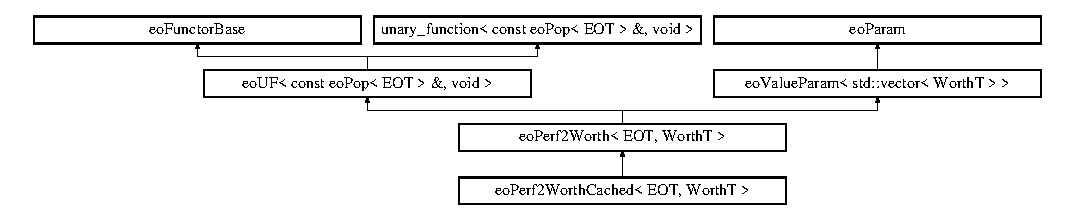
\includegraphics[height=2.52252cm]{classeo_perf2_worth_cached}
\end{center}
\end{figure}
\subsection*{Public Member Functions}
\begin{CompactItemize}
\item 
{\bf eo\-Perf2Worth\-Cached} (std::string \_\-description=\char`\"{}Worths\char`\"{})\label{classeo_perf2_worth_cached_a0}

\item 
void {\bf operator()} (const {\bf eo\-Pop}$<$ {\bf EOT} $>$ \&\_\-pop)
\begin{CompactList}\small\item\em Implementation of the operator(), updating a cache of fitnesses. \item\end{CompactList}\item 
virtual void {\bf calculate\_\-worths} (const {\bf eo\-Pop}$<$ {\bf EOT} $>$ \&\_\-pop)=0\label{classeo_perf2_worth_cached_a2}

\begin{CompactList}\small\item\em The actual virtual function the derived classes should implement. \item\end{CompactList}\item 
virtual void {\bf sort\_\-pop} ({\bf eo\-Pop}$<$ {\bf EOT} $>$ \&\_\-pop)\label{classeo_perf2_worth_cached_a3}

\begin{CompactList}\small\item\em Sort population according to worth, will keep the worths and fitness\_\-cache in sync with the population. \item\end{CompactList}\item 
virtual void {\bf resize} ({\bf eo\-Pop}$<$ {\bf EOT} $>$ \&\_\-pop, unsigned sz)\label{classeo_perf2_worth_cached_a4}

\end{CompactItemize}
\subsection*{Private Attributes}
\begin{CompactItemize}
\item 
std::vector$<$ typename EOT::Fitness $>$ {\bf fitness\_\-cache}\label{classeo_perf2_worth_cached_r0}

\end{CompactItemize}


\subsection{Detailed Description}
\subsubsection*{template$<$class EOT, class Worth\-T = typename EOT::Fitness$>$ class eo\-Perf2Worth\-Cached$<$ EOT, Worth\-T $>$}

Perf2Worth with fitness cache. 



Definition at line 111 of file eo\-Perf2Worth.h.

\subsection{Member Function Documentation}
\index{eoPerf2WorthCached@{eo\-Perf2Worth\-Cached}!operator()@{operator()}}
\index{operator()@{operator()}!eoPerf2WorthCached@{eo\-Perf2Worth\-Cached}}
\subsubsection{\setlength{\rightskip}{0pt plus 5cm}template$<$class EOT, class Worth\-T = typename EOT::Fitness$>$ void {\bf eo\-Perf2Worth\-Cached}$<$ {\bf EOT}, Worth\-T $>$::operator() (const {\bf eo\-Pop}$<$ {\bf EOT} $>$ \& {\em \_\-pop})\hspace{0.3cm}{\tt  [inline, virtual]}}\label{classeo_perf2_worth_cached_a1}


Implementation of the operator(), updating a cache of fitnesses. 

Calls the virtual function calculate\_\-worths when one of the fitnesses has changed. It is not virtual, but derived classes can remove the fitness caching trough the third template element 

Implements {\bf eo\-UF$<$ const eo\-Pop$<$ EOT $>$ \&, void $>$} {\rm (p.\,\pageref{classeo_u_f_a1})}.

Definition at line 125 of file eo\-Perf2Worth.h.

The documentation for this class was generated from the following file:\begin{CompactItemize}
\item 
eo\-Perf2Worth.h\end{CompactItemize}
